
\subsubsection{1.1.2 les thématiques des versets
médinois
}

- le thème d'Abraham comme «~Père des croyants~» où Abraham est dit
d'une part \emph{ḥanīf}, c'est-à-dire monothéiste exclusif, mais aussi
\emph{muslim}, c'est-à-dire soumis, abandonné à Dieu, et ni juif ni
chrétien, date de la période médinoise.

(S. 3, 67-68).

«~Abraham n'était ni juif ni chrétien, mais il était un monothéiste
exclusif, abandonné à Dieu~; il n'était pas au nombre des polythéistes.
Les hommes les plus proches d'Abraham sont vraiment ceux qui l'ont
suivi, ainsi que ce Prophète et ceux qui ont cru~».
\marginpar{ \footnotesize This is a margin note using the geometry package, set at 5cm 
vertical offset to the first line it is typeset.}


\foreignlanguage{arabic}{لَكِنْ
}
test
\TArabe{مَا كَانَ إِبْرَاهِيمُ يَهُودِيًّا وَلَا نَصْرَانِيًّا وَلَكِنْ
كَانَ حَنِيفًا مُسْلِمًا وَمَا كَانَ مِنَ الْمُشْرِكِينَ إِنَّ أَوْلَى
النَّاسِ بِإِبْرَاهِيمَ لَلَّذِينَ اتَّبَعُوهُ وَهَذَا النَّبِيُّ
وَالَّذِينَ آَمَنُوا وَاللَّهُ وَلِيُّ الْمُؤْمِنِينَ}




\begin{otherlanguage}{arabic}
{مَا كَانَ إِبْرَاهِيمُ يَهُودِيًّا وَلَا نَصْرَانِيًّا وَلَكِنْ
كَانَ حَنِيفًا مُسْلِمًا وَمَا كَانَ مِنَ الْمُشْرِكِينَ إِنَّ أَوْلَى
النَّاسِ بِإِبْرَاهِيمَ لَلَّذِينَ اتَّبَعُوهُ وَهَذَا النَّبِيُّ
وَالَّذِينَ آَمَنُوا وَاللَّهُ وَلِيُّ الْمُؤْمِنِينَ}
\end{otherlanguage}

Ce verset a bien sûr donné lieu à de multiples commentaires. Il est
souvent interprété dans le sens où Abraham est dépositaire de la
religion originelle avant son altération par les juifs et les chrétiens. \cite{Ben62}
Souvent ne veut pas pour autant dire toujours. Il y a d'autres
lectures\ldots{} \sn{\cite{Ben62}}

\begin{figure}
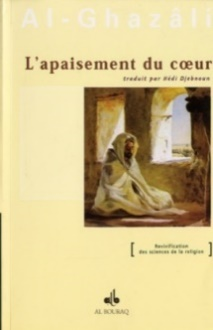
\includegraphics{Images/image002.jpg}
\sidecaption{essai}
\end{figure}


\begin{table}[h!]
\resizebox{\textwidth}{!}{%
\small
\begin{tabular}{p{2cm}p{4cm}p{4cm}}
\toprule
essai & essai & essai \\
\midrule
essai & essai & essai \\
\bottomrule

\end{tabular}%
}
\sidecaption{essai}
\end{table}

\begin{longtable}{p{6cm}p{6cm}}
\toprule
\endhead
«~Quiconque obéit au Messager obéit certainement à Allah~». 
&\TArabe{ مَّن
يُطِعِ الرَّسُولَ فَقَدْ أَطَاعَ اللَّهَ }\\
\bottomrule
\end{longtable}